\section{微博的四种采集}

微博把四种采集都做全了，用它能讲清同一个数据源节点的四种形态。打开“\texttt{测试：微博}”，画布上是四条并排的链，加一条关掉的备用链。

\begin{figure}[H]\centering
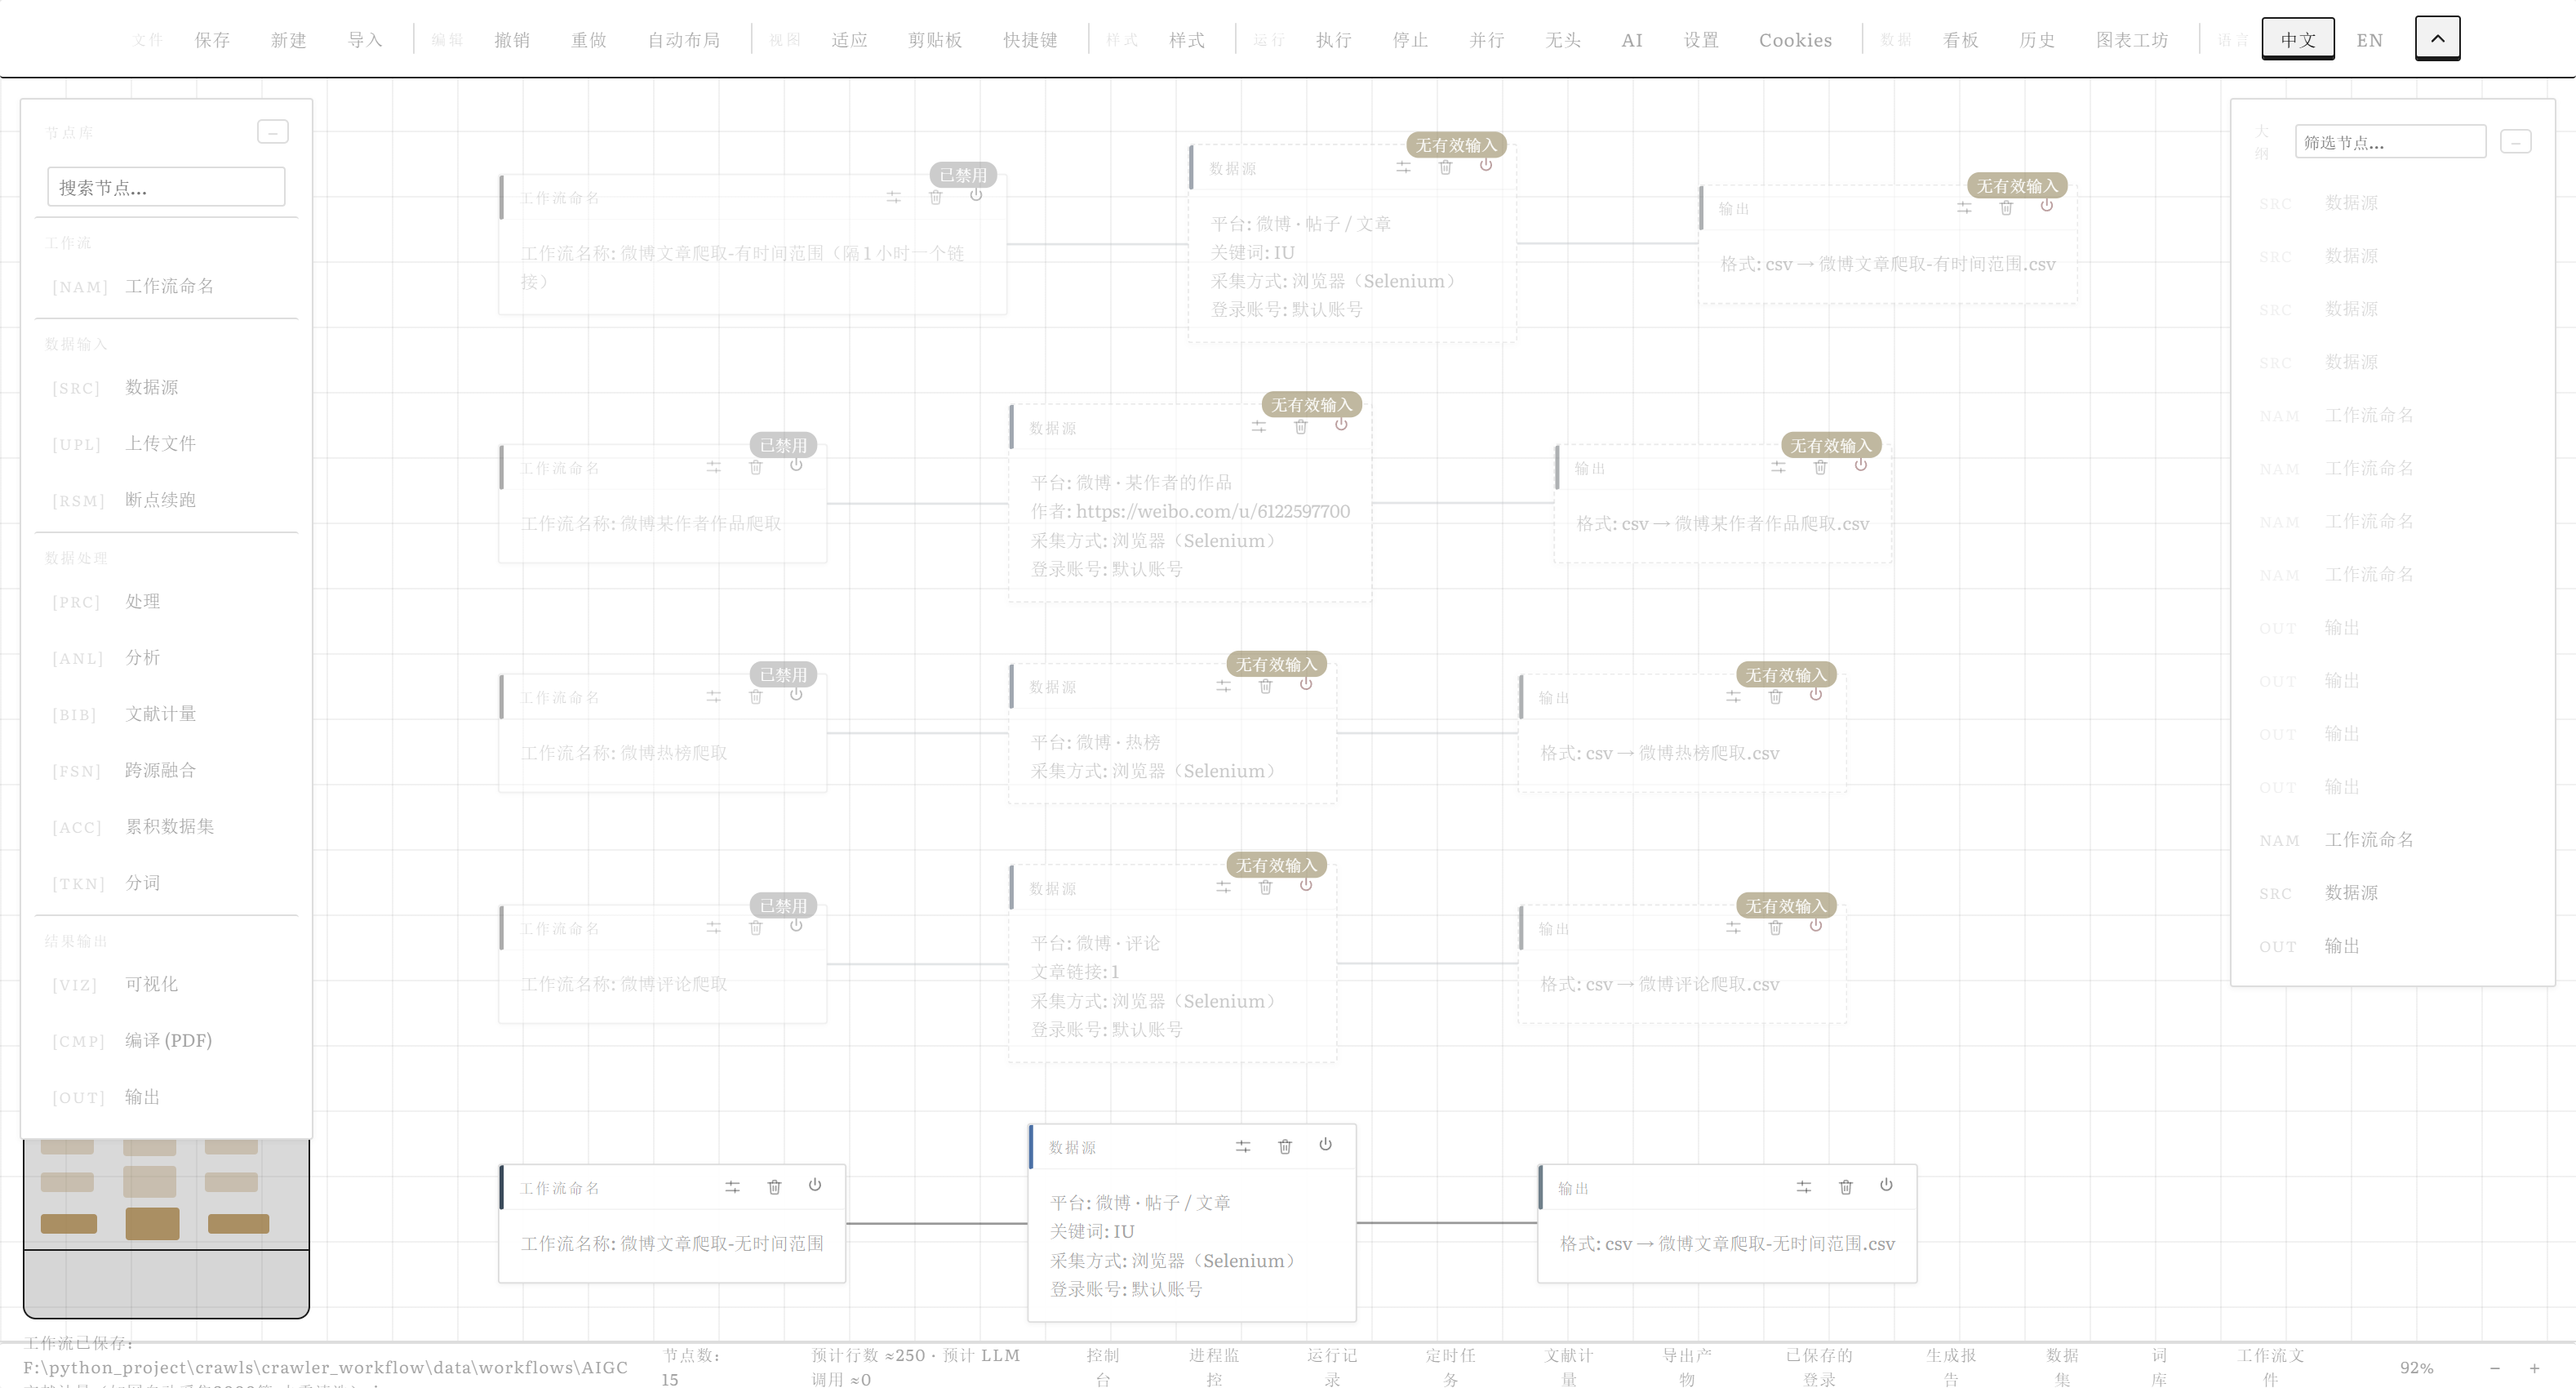
\includegraphics[width=0.9\textwidth]{wb-canvas.png}
\caption{微博四条链：关键词、作者、热搜、评论}
\label{fig:wb-canvas}
\end{figure}

\subsection{关键词与时间范围}

第一条链按关键词采。平台“\texttt{微博}”，内容“\texttt{帖子}”，关键词填 \texttt{IU}，
开始时间 \texttt{2026-01-01}，结束时间 \texttt{2026-09-26}，展开全文打勾，目标数量 50。
微博按时间窗翻页，填了两端就只在这个区间里走。展开全文会点进每条取正文，慢但完整。

\begin{figure}[H]\centering
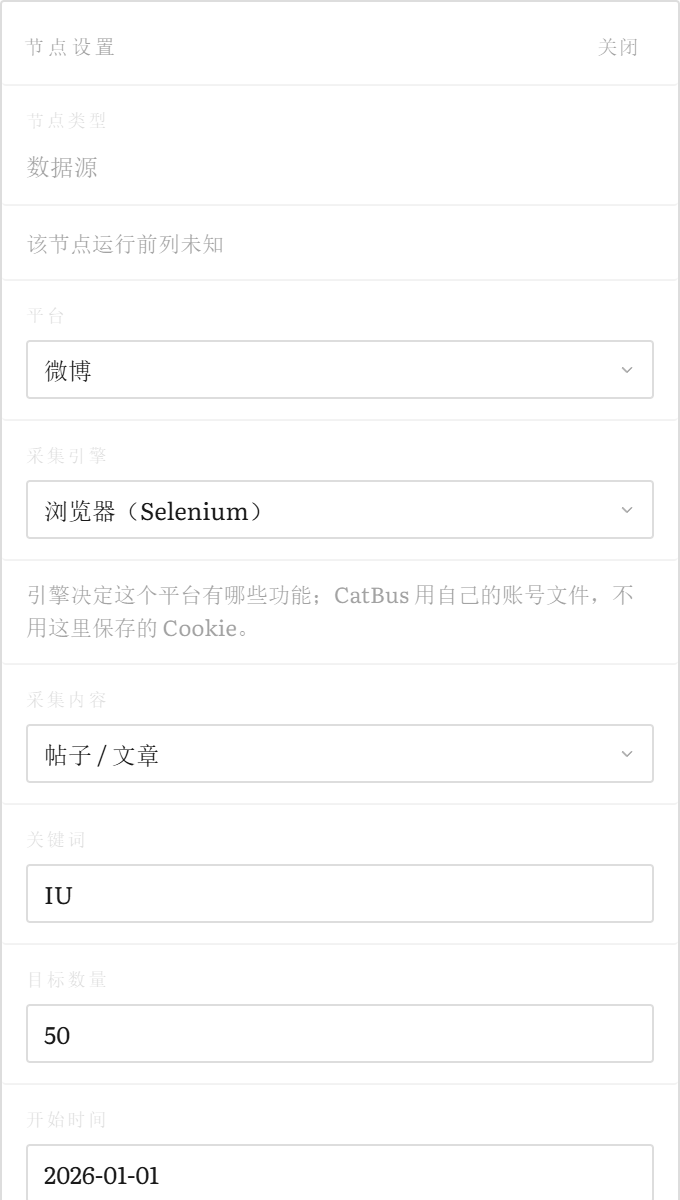
\includegraphics[width=0.31\textwidth]{wb-keyword.png}
\caption{关键词模式：时间范围与展开全文}
\label{fig:wb-keyword}
\end{figure}

时间窗有代价，站点翻得越深越慢，数量不用填太大。程序一路翻到站点给不出下一页为止。

\subsection{作者作品}

第二条链把内容换成“\texttt{某作者的作品}”，作者填主页链接或者那串数字 UID。作者这一栏要么填完整链接，要么填纯数字，
填昵称不行，填错时程序会拒绝并说明要哪种形式。作品列表从作者主页自己的接口一页页取，不需要登录也能看到公开部分。

\subsection{热搜}

第三条链选“\texttt{热搜}”。这一项不需要登录，采到的是当下这一刻的榜单，带精确整数热度。
即时榜重复运行会把同一时刻的榜再存一遍，要不要重采看用途。

\subsection{评论}

第四条链采评论，文章链接写一条微博地址，每篇单独文件打勾。评论节点与别的平台共用一套面板：
能设评论时间筛选、是否包含回复、条数上限，上游是表时还能按某一列逐行喂链接。

\begin{figure}[H]\centering
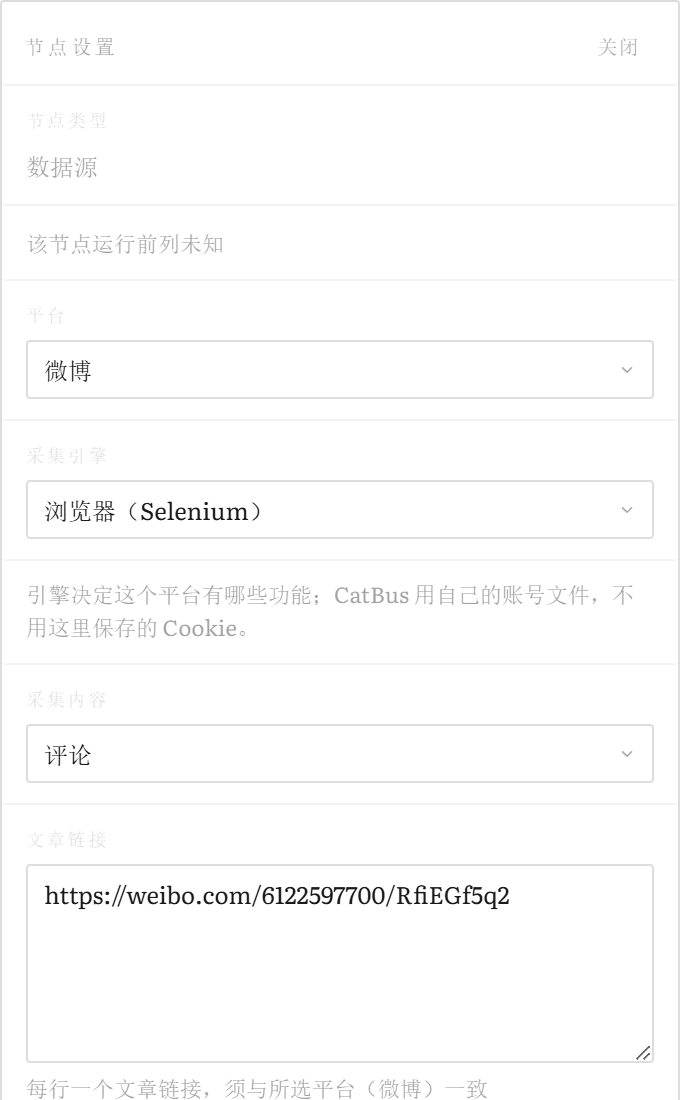
\includegraphics[width=0.31\textwidth]{wb-comment.png}
\caption{评论节点：时间筛选与条数上限}
\label{fig:wb-comment}
\end{figure}

有些平台、有些视频不发布评论者的 IP 属地，评论地区这一列可能是空的。画布里只要出现评论节点，运行前会提示一次，纯搜索的画布不会打扰。

\section{抖音作者、评论与两路分析}

这一条链把采集和模型接在一起。打开“\texttt{测试：抖音}”。三段：作者作品、评论、两路情感分析。

\begin{figure}[H]\centering
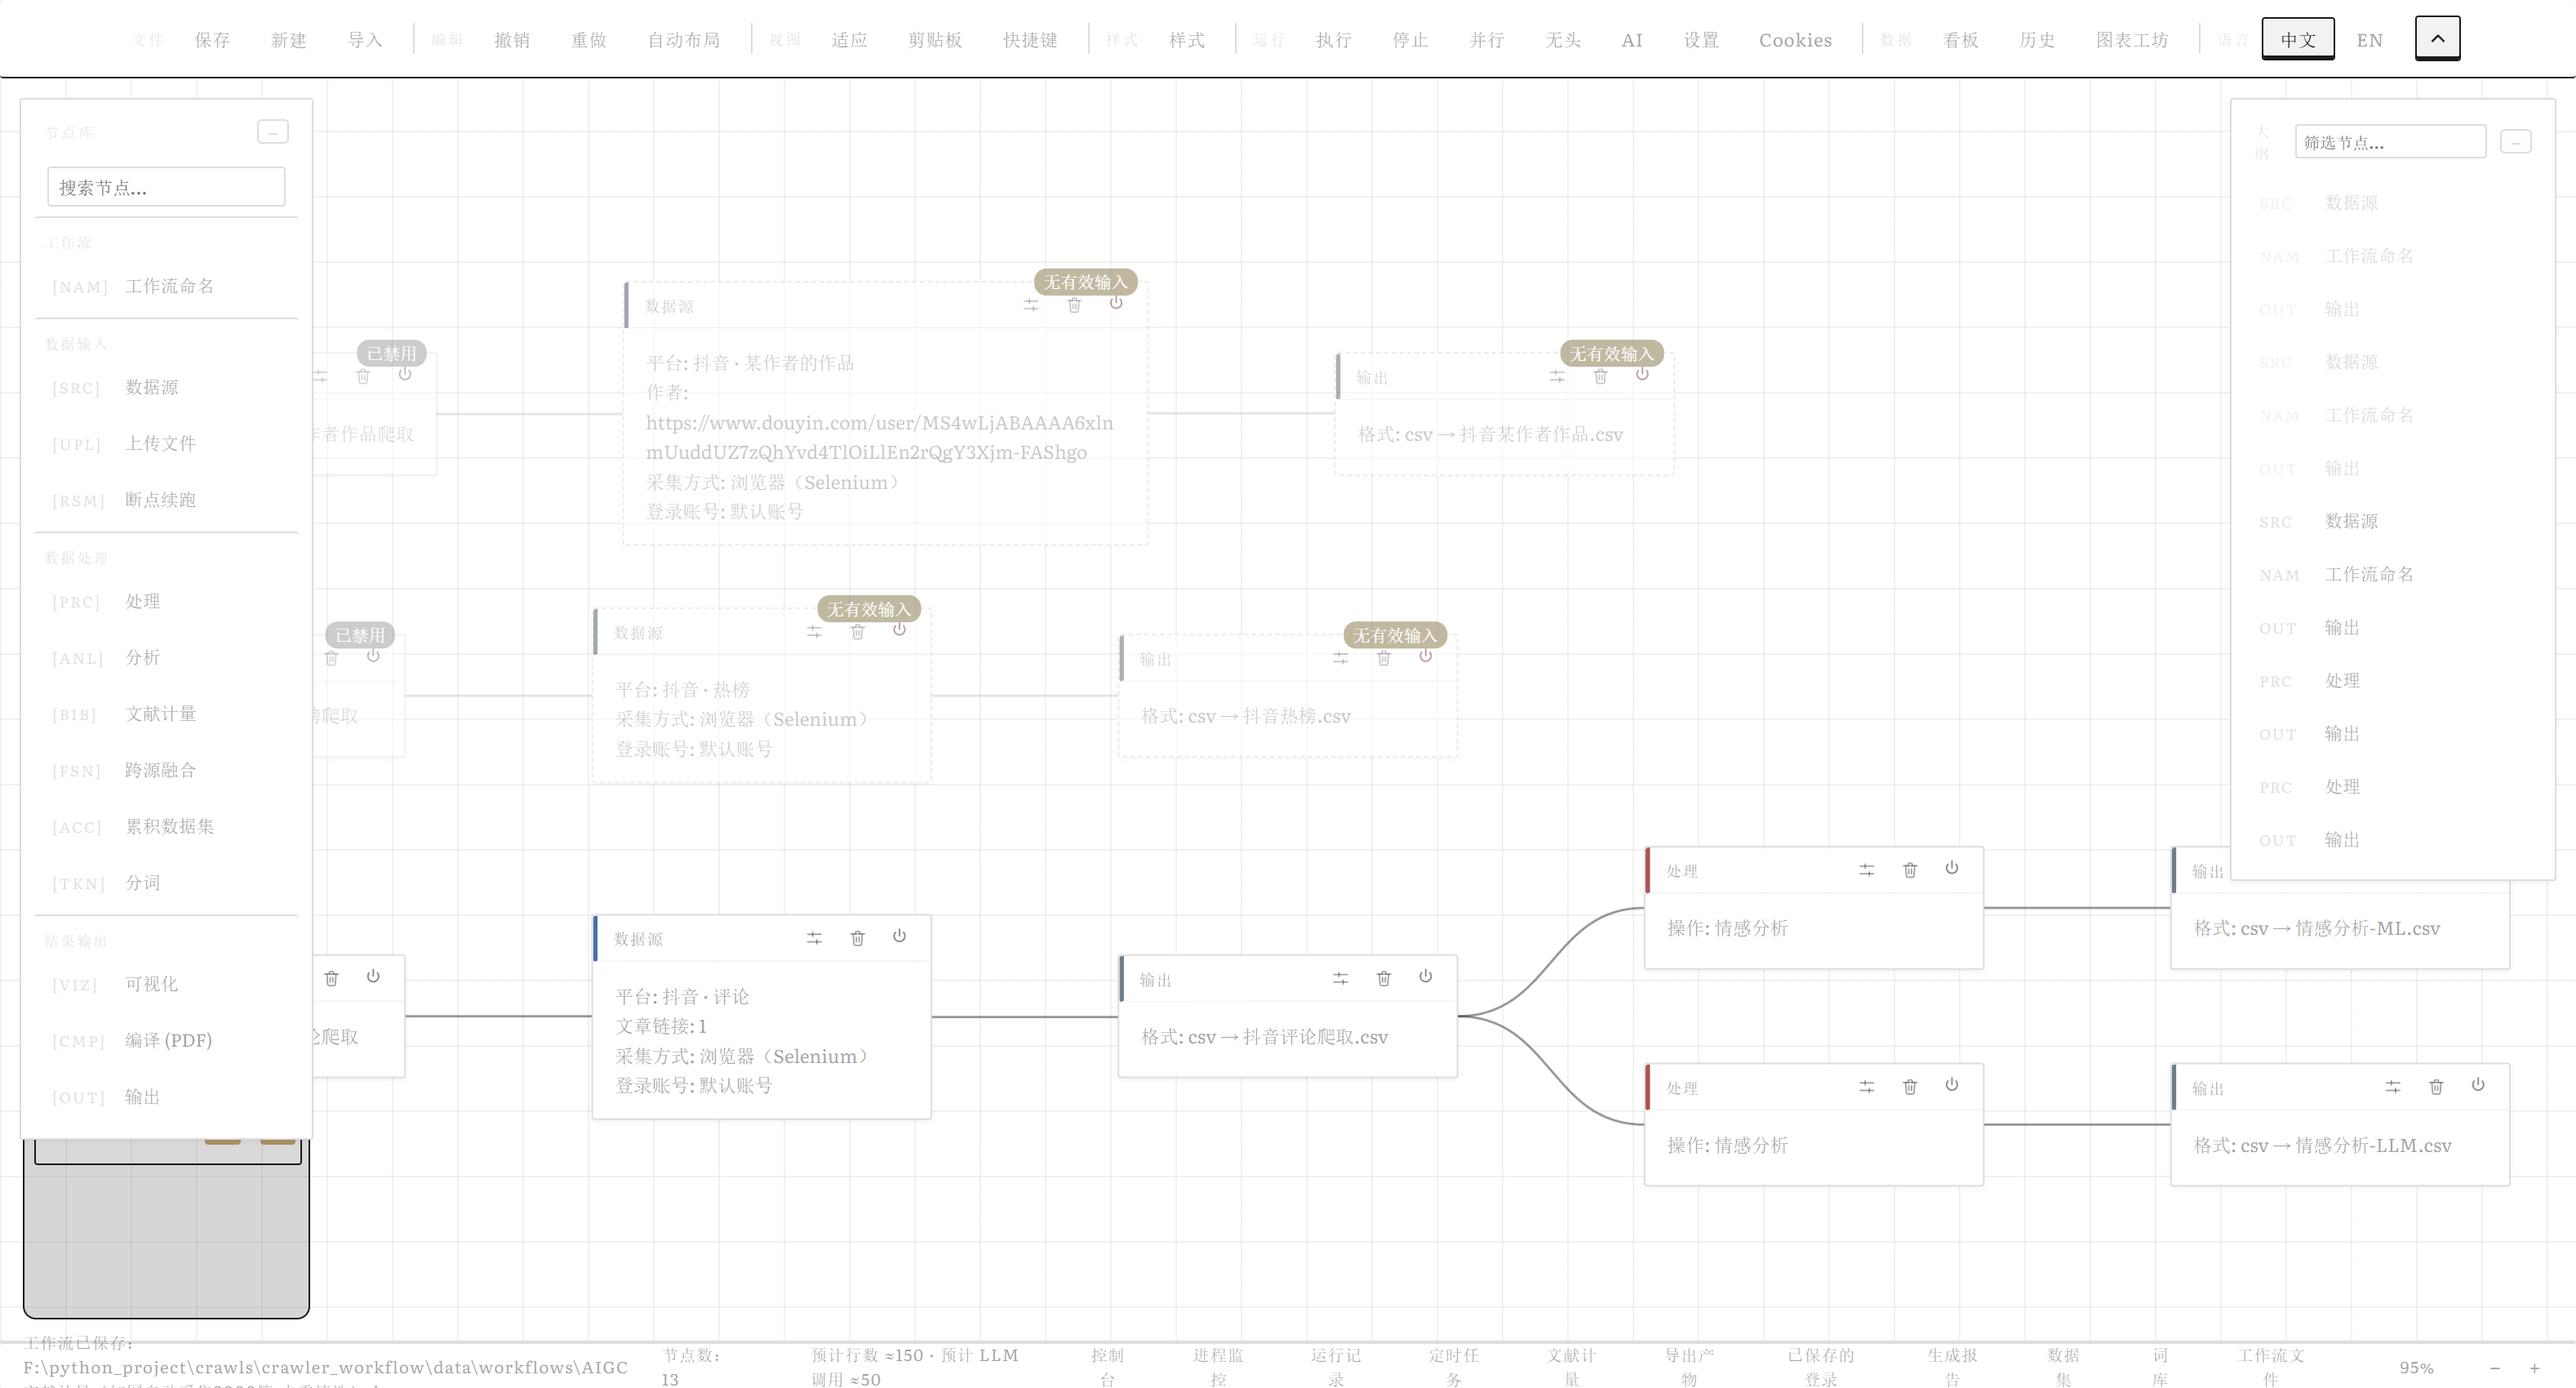
\includegraphics[width=0.98\textwidth]{dy-canvas.png}
\caption{抖音三段：作者作品、评论、两路情感分析}
\label{fig:dy-canvas}
\end{figure}

数据源选“\texttt{抖音}”，内容“\texttt{某作者的作品}”，作者填主页链接。抖音只认链接里那串 \texttt{sec\_uid}，填昵称会被拒收。
作品网格在站内用遮罩打开，程序读遮罩里的卡片，不逐条跳转。第二个数据源采评论，链接写一条视频地址，
评论面板要一路滚到底，楼层号按站点给出的顺序编号。

后面两个“\texttt{处理}”节点都是情感分析，用同一个文本列，区别只在分析模式：一路传统机器学习，一路大模型。
一次跑完就能对比两种模式的结论、费用与耗时。

\begin{figure}[H]\centering
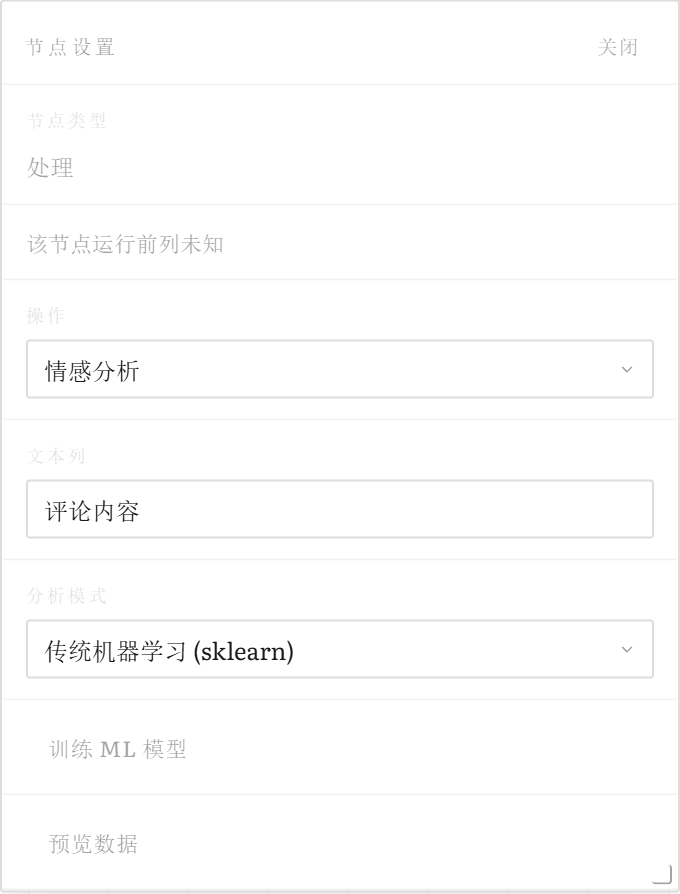
\includegraphics[width=0.31\textwidth]{dy-sentiment.png}
\caption{情感分析节点：操作、文本列、分析模式三行必填}
\label{fig:dy-sentiment}
\end{figure}

BERT 跑不起来时节点自动降级到机器学习，并在控制台写明这一轮实际用的是哪种，不会把降级结果说成 BERT。
大模型那一路逐行调用，日志里能看到每批保存了多少行。跑完两个输出文件分别是“\texttt{情感分析-ML.csv}”与“\texttt{情感分析-LLM.csv}”，
同一批评论两套结论，可以直接拿去做对比图。

\section{知乎关键词到词云}

这一条最短，覆盖采集到出图的全程。打开“\texttt{测试：图表可视化}”。

\begin{figure}[H]\centering
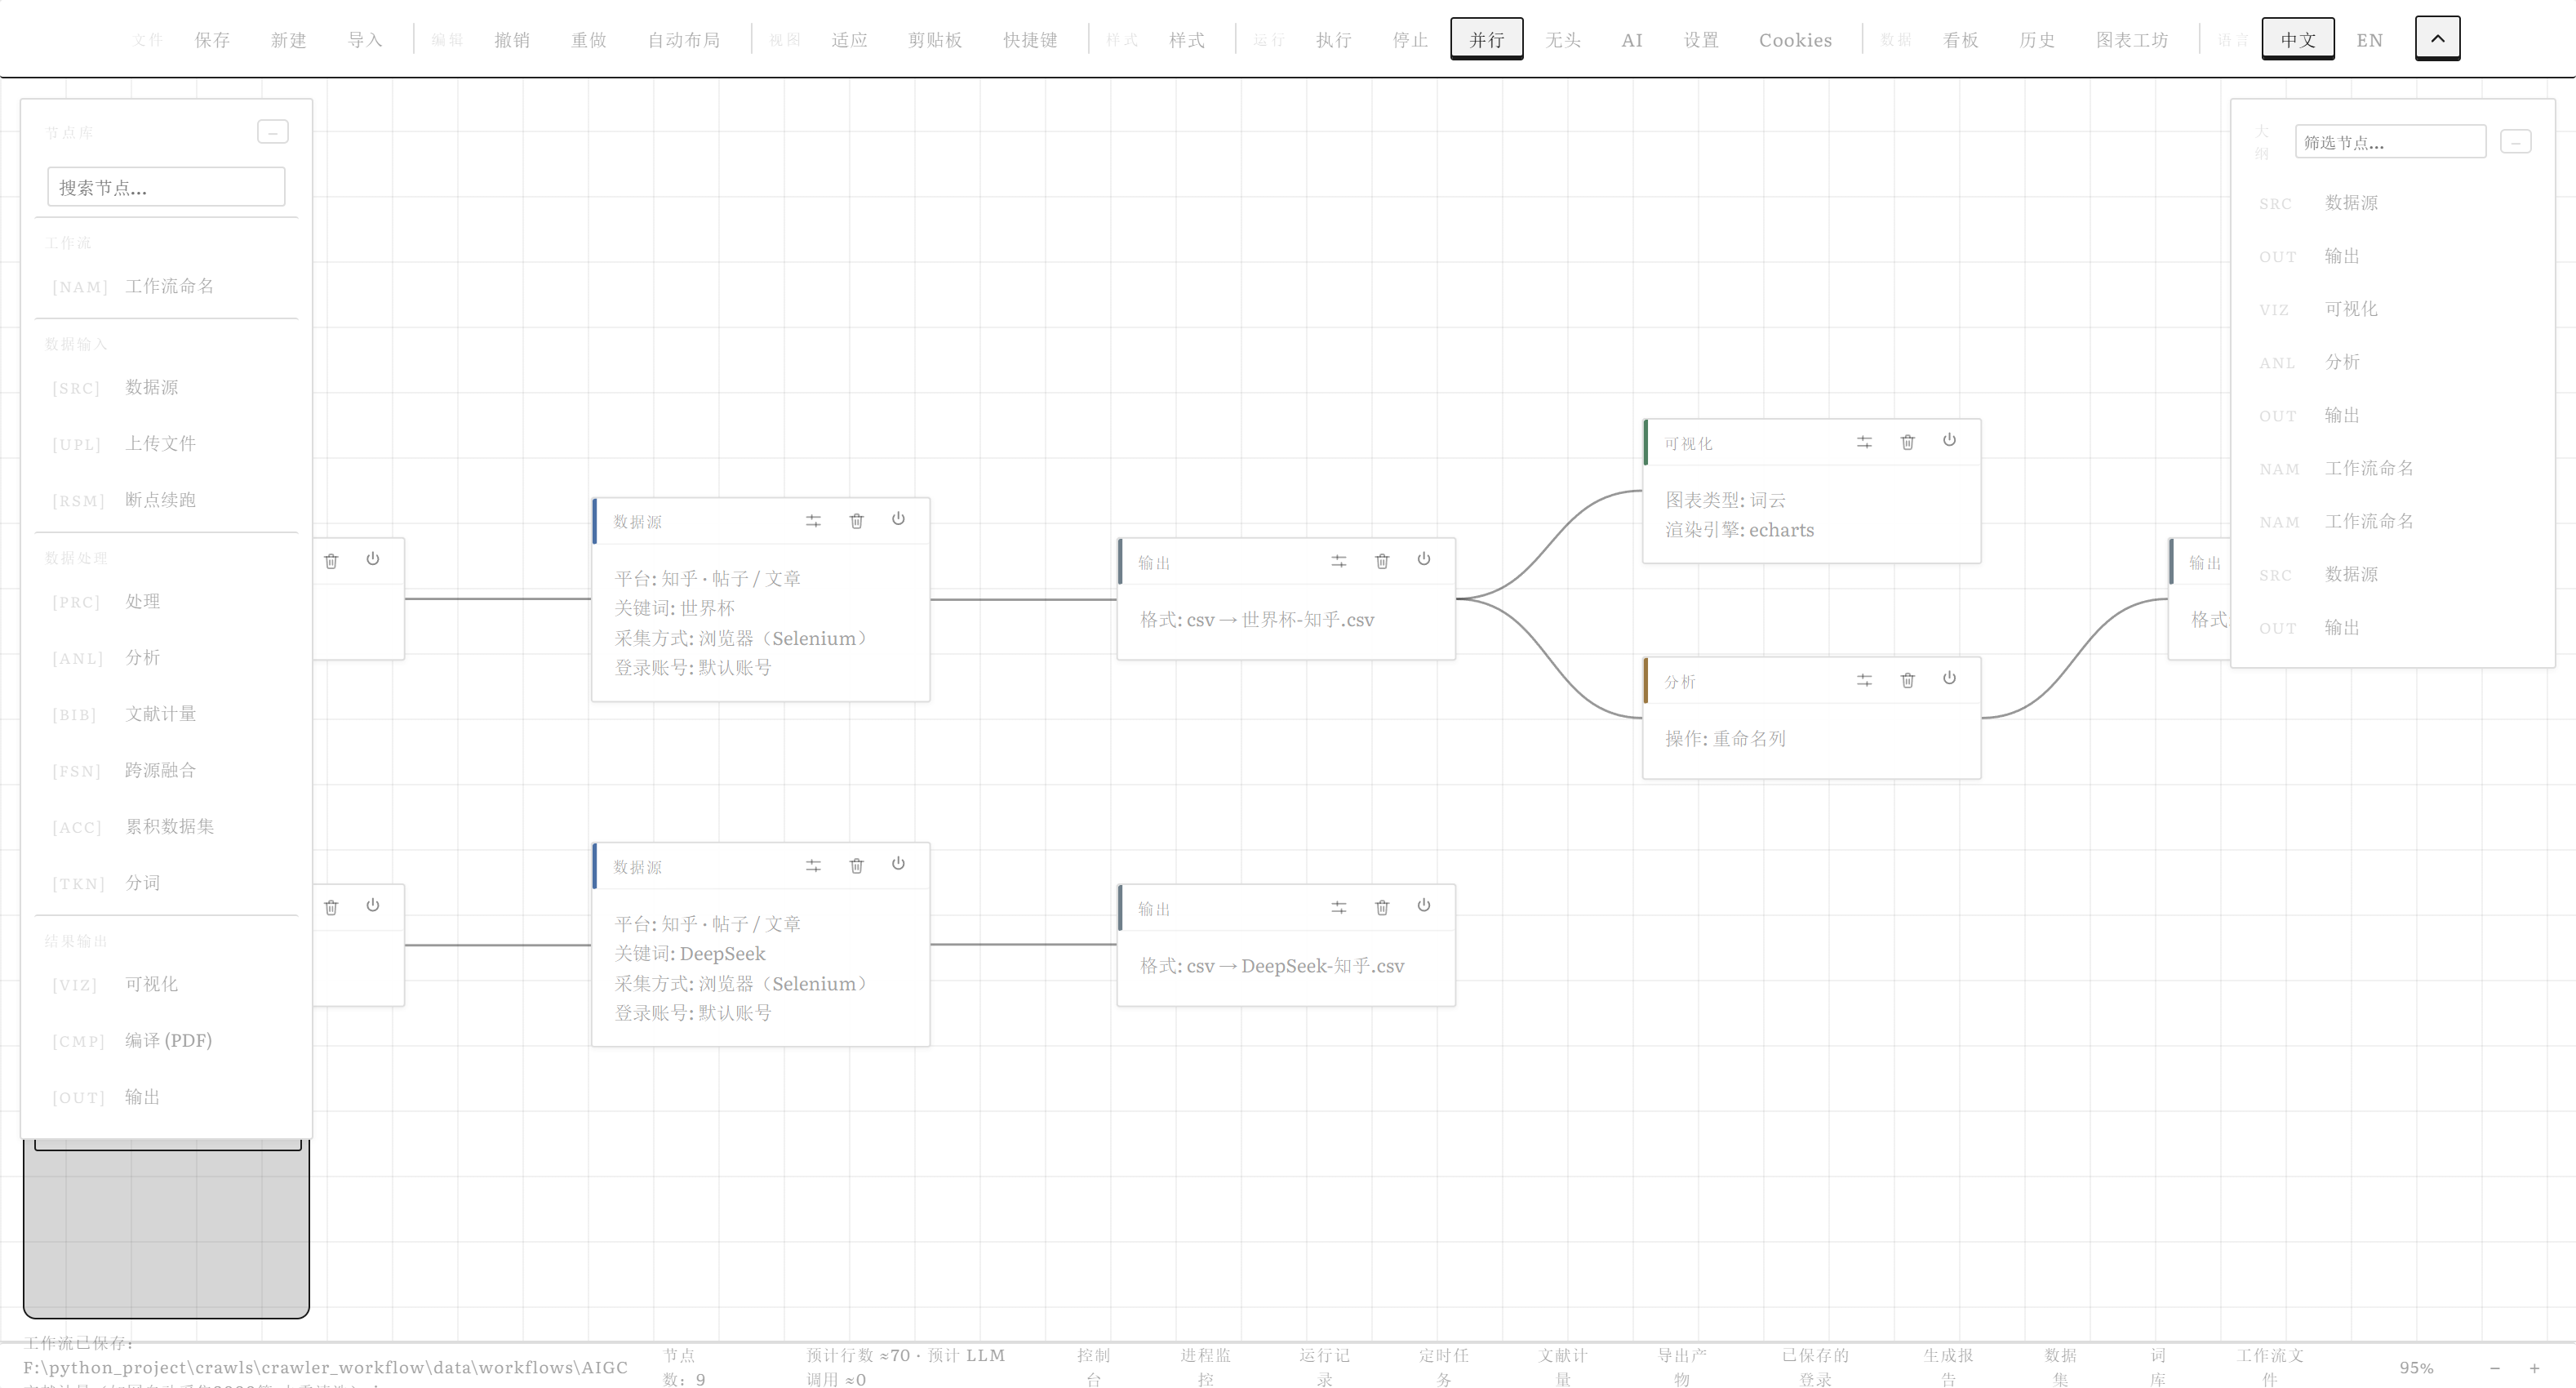
\includegraphics[width=0.98\textwidth]{zh-canvas.png}
\caption{知乎关键词采下来，改列名，出一张词云}
\label{fig:zh-canvas}
\end{figure}

数据源选“\texttt{知乎}”，内容“\texttt{帖子与文章}”，关键词“\texttt{世界杯}”，目标 20 条，展开全文打勾。
知乎搜索卡片只给摘要，勾了才会把全文读进来。

中间“\texttt{分析}”节点的操作是“\texttt{重命名列}”，把“\texttt{作者}”改成“\texttt{发帖人}”。上游列名不合适，
或者下游要按固定列名读，就在这里改一次，后面全部统一。

最后一个“\texttt{可视化}”节点，图表类型“\texttt{词云}”，引擎 \texttt{ECharts}，横轴字段“\texttt{正文}”，分词打勾。
词云直接吃原文，自己切词，不必先过“处理 → 分词”。

\begin{figure}[H]\centering
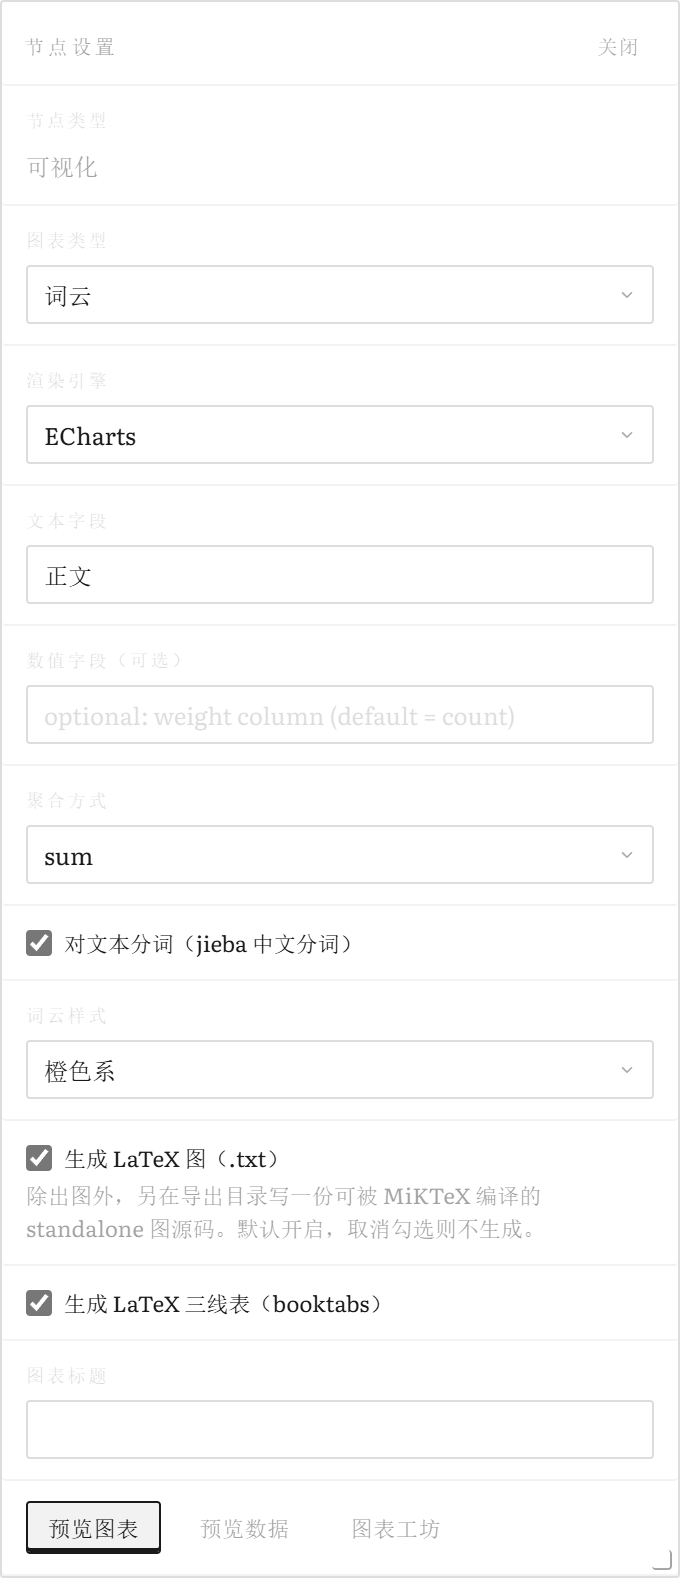
\includegraphics[width=0.31\textwidth]{zh-visualize.png}
\caption{可视化节点：图表类型、引擎、LaTeX 选项、标题}
\label{fig:zh-visualize}
\end{figure}

面板底部三个按钮：预览图表看效果，预览数据看这张图的输入表，图表工坊把这份数据送进作图台。跑过一次以后才有内容可看。

\section{采集疑难}

问题大多出在登录、速度、并发三件事上。

\subsection{登录过期}

症状是跑到一半跳到登录页，日志写登录墙。打开“\texttt{Cookies}”，选平台与账号，重新存一份再验证。
已经采到的行不会丢，重新执行会从断点接上。微博有一种假登录墙，搜索时页面会闪一下扫码页再弹回结果，
程序等页面稳定再判断，真掉线才报错。

\subsection{同一平台并行}

同一份浏览器目录同一时刻只能开一个。画布上有两条以上同平台的链又勾了并行，运行前会问你一次：
排队跑、换账号或者串行。设置里“\texttt{同平台排队采集}”打开就是真排队，一次只跑一条，前一条完才轮到下一条；
“\texttt{同平台错峰间隔}”给不排队的情况留一个几秒的缓冲。

\subsection{采得慢或者采不到}

站点风控会限制频率。设置里的“\texttt{慢速采集}”打开以后每轮操作之间多停一会儿，不是万能，但比硬撞好。
海外平台还要网络通。画布上出现海外平台时，运行前会问一句外网通不通，不通先挂上再跑，别把超时当站点改版。

\subsection{采到的行数不够}

看日志最后一句。写的是站点给出的最后一页，就是真到底了；写的是风控、登录、超时，就是被拦住了。
换时间、换账号、开慢速再试。程序不会把短表默默交给你，一定说明为什么短。

\subsection{第二套采集后端}

有些平台只能用 CatBus，比如快手、TikTok、京东、淘宝、闲鱼，这类平台的采集引擎下拉里只有它。
CatBus 要本机装 Node 与它的适配器，缺哪一样都按名字说清是缺哪一样，不会给一张空表然后标成完成。
它的登录门与浏览器那套分开，用自己的账号文件，登录状态也不与 Cookie 面板混用。
